\documentclass[twocolumn,10pt]{article}

\usepackage[a4paper,hmargin=1.5cm,vmargin=2.5cm,]{geometry}
\setlength{\columnsep}{0.7cm}
\usepackage{palatino}
\usepackage{graphicx}
\usepackage[utf8]{inputenc}
\usepackage{hyperref}
\usepackage{minted}
\usemintedstyle{colorful}
\usepackage[font=small,labelfont=bf]{caption}
\urlstyle{same} % no tt font for URLs
\newcommand{\blockade}{\rule{3em}{0.7em}}  %% Marker for things to change before submission

\usepackage{natbib}
\bibliographystyle{genome_research}
\setcitestyle{aysep={}} 

\usepackage{xcolor}
\hypersetup{
    colorlinks,
    linkcolor={blue!50!black},
    citecolor={blue!50!black},
    urlcolor={blue!50!black}
}

\begin{document}

\setcounter{secnumdepth}{0}


\twocolumn[{%
\centering
\textbf{\Large R/LinkedCharts: A novel approach for simple but powerful interactive data analysis}
\vspace{1.5ex}

Svetlana Ovchinnikova and Simon Anders\\
{\footnotesize Center for Molecular Biology of the University of Heidelberg, Germany}
\vspace{1.5ex}

24 January 2020
\vspace{6ex}
}]

\section{Abstract}
In exploratory data analysis, one usually jumps back and forth between visualizations that provide overview of the whole data and others that dive into details. In data quality assessment, for example, it might be very helpful to have one chart showing a summary statistic for all samples, and clicking on one of the data points would display details on this sample in a second plot. Setting up such interactively linked charts is usually cumbersome and time-consuming to use them in ad hoc analysis. We present R/LinkedCharts, a framework  that renders this tasks radically simple: Producing linked charts is as quickly done as is producing conventional static plots in R, requiring a data scientist to write only very few lines of simple R code to obtain complex and general visualization. We expect that the convenience of our new tool will enable data scientists and bioinformaticians to perform much deeper and more thorough EDA with much less effort. Furthermore, R/LinkedCharts apps, typically first written as quick-and-dirty hacks, can also be polished to provide interactive data access in publication quality, thus contributing to open science.

\section{Introduction}

Problem of effective visualization has been there since the first reported experiment results. Continuously growing amount and complexity of available data over the last decades made it a challenging issue \citep{fisher_2017}. For a while the only available way to tackle the problem was to come up with more elaborate types of plots imploying colour, shape, transparensy and other visual aspects to combine multiple layers of information \citep{keahey_2013}. Yet, there are certain limits to how much information one can grasp from a static image. Excessive details and overcomplexity make visualization less interprateable. Thus a researcher is forced to make a decision on what information to keep when preparing figures for a paper or any other kind of report. From one hand, it is a good thing, since often data contains plenty of noise and information that is irrelevant to the point one tries to make. From the other hand, it may be complicated to make sure, that nothing of importance is missing in the graphical representation.

With the advance of mordern technologies, interactive visualisation emerged to offer a solution to this problem. In an interactive figure there is no need to make all aspects visible simultaneously or highlight everything of importance at once. Instead user is allowed to explore the figure in a quick and intuitive manner, concentrating at a time on the most interesting or suspicsious parts of the plot. Numerous tools now provide means of creating interactive visualizations not only for research, but for any area that involves data analisys and presentation of any sort \citep{caldarola_2017}. With their help one may avoid overburdening of figures without a need to put some information aside.

The advantage of interactivity lies beyond just simplifying navigation through big massives of data. When adding small changes to a plot takes just a click or two, it urges a researcher not to put aside ideas or concerns and thus go through the data more thoroughly. At the same time a possibility for readers to check conclusions and claims of a paper on the fly, without going through all the script and analysis, makes the paper more credible. Therefore, we believe that further integration of interactive tools in a researchers' routine can strongly improve quality of studies.

Today many papers offer an interactive resource as a way to present their data and results. Though these visualizations are often useful and provide a comprahensive insight into the data, they generally serve presentation purposes only. This means that only after completing main work on the project, researches spend a couple of days to deploy a nice interactive app to share their data and results with the scientific community. We, however, believe, that interactivity should also be used in every day tasks to facilitate data exploration. To this end, the tool to produce interactive apps should be both simple and highly customizeable.

Simplicity should serve as incentive to use interactivity whenever there is a smallest hint that it may be useful. If a tool is too complicated, one may prefer to do most of the analysis by more habitual static means, and wait for a special occasion when it's worthwhile to invest time into designing an interactive app. It should also be similar in design to most common visualization means, since tools with too specific interface tend to be used by people with more extensive programming skill. Even if a researcher with less expertise in coding has an eager-to-help colleague, he or she may be unwilling to ask for an assistance in minual every day tasks and wait for something big.

At the same time, an attempt to simplify a tool may result in hardcoding and presetting too many parameters. As a result, a simple-to-use tool can be applied to a single task it was designed for and any attempt of custamization, if at all possible, requires a considerable effort. Yet, it may be useful if one doesn't try to force a research problem in the predefined mould of a certain tool, but rather makes tool to fit a problem. This requires a reasonable degree of flexibility.

With the LinkedCharts, we've tried to find a ballance between the two goals of a tool for interactive data exploration. It requires only basic knowledge in R or JavaScript to produce fully functional apps that can be used for \emph{ad hoc} analysis. With a little more effort one can make a nicer looking app and customize most of commonly used plot settings (such as colours, labels, axes, etc.). And finally, with the time and skills that is generally required for the same task, one can use LinkedCharts to make a presentable app deployed on a server. Since the library is JavaScript based, it can be combined with various existing web solutions. One can also write cutom scripts that will change even hardcoded aspects of the library without making changes to the source code, thus making LinkedCharts extremely flexible. 

LinkedCharts is not fixed on any specific task. It is rather a toolbox and its blocks can be combined in any manner the same way as one combines plots for a complex paper figure. All block share the same interface and very similar interactivity capabilities, which means that understanding one of them is enough to grasp the entire concept of LinkedCharts.

With all these, we hope that LinkedCharts can become a useful asset for a scientific community that can be used both for everyday routine and for presenting one's reasearch to a greater audience. LinkedCharts available as an R package (can be downloaded from CRAN) and as a JavaScript library. This paper is focused on R implementation of LinkedCharts. 

\section{Results}
\subsection{Linking charts}

The main consept behind LinkedCharts is connecting to or more plots together so that manipulation with one of them affect the others. This process is what ``linked'' in ``LinkedCharts'' stands for. It can be better explained with a simple example based on data from 

As an example, let us think about a routine differential expression analisys. A question that is often arises as a part of some bigger study is how the two groups of samples or cells are different. Here and in the live version in the supplement, we've used data from [reference]. In this study, from each of 17 patients with oral cancer three samples were taken: one of normal tissue, one of tumour and one of displasia tissue. mRNA from all these samples was sequenced to obtain gene expression values. Now, one may want to know what genes are significantly different between, let say, normal and cancerous tissues. Many packages offer functions to answer this question and for this example it is not important, which one to use. We've applied function \mintinline{R}{voom} from the ``limma'' package. To explore results of this function it is common to make an MA-plot with the average gene expression on the x-axis and log fold change between the two groups on the y-axis. It can be also convenient to have such a plot next to another that shows expression of the selected gene across all the samples. This can be easily done with R/LinkedCharts.

Let say, normalized counts are stored as matrix in the \mintinline{R}{normCounts}. \mintinline{R}{sampleTable} is a \mintinline{R}{data.frame} with information about samples: patient IDs, tissue types, etc. \mintinline{R}{voomResult} is an output of the \mintinline{R}{voom} function from the ``limma'' package. This data frame for each gene contains its average expression, log fold change and p-value for significance of the expression difference.

Here, how one can make an app with these two linked plots using the R/LinkedCharts library.

\begin{minted}{R}
openPage(layout = "table1x2")
gene <- 1

lc_scatter(dat(
   x = AveExpr,
   y = tissuetumour,
   colour = ifelse(adj.P.Val < 0.1, 
                   "red", "black"),
   on_click = function(k) { 
      gene <<- k
      updateCharts("A2") 
   }),
"A1", with = voomResult)

lc_scatter(dat(
   x = patient,
   y = normCounts[gene, ],
   colourValue = tissue, 
   logScaleY = 10),
"A2", with = sampleTable)
\end{minted}

The app produced by this code and the data to reproduce it can be found in the supplement.


\subsection{Structure and linking}
\begin{figure*}
	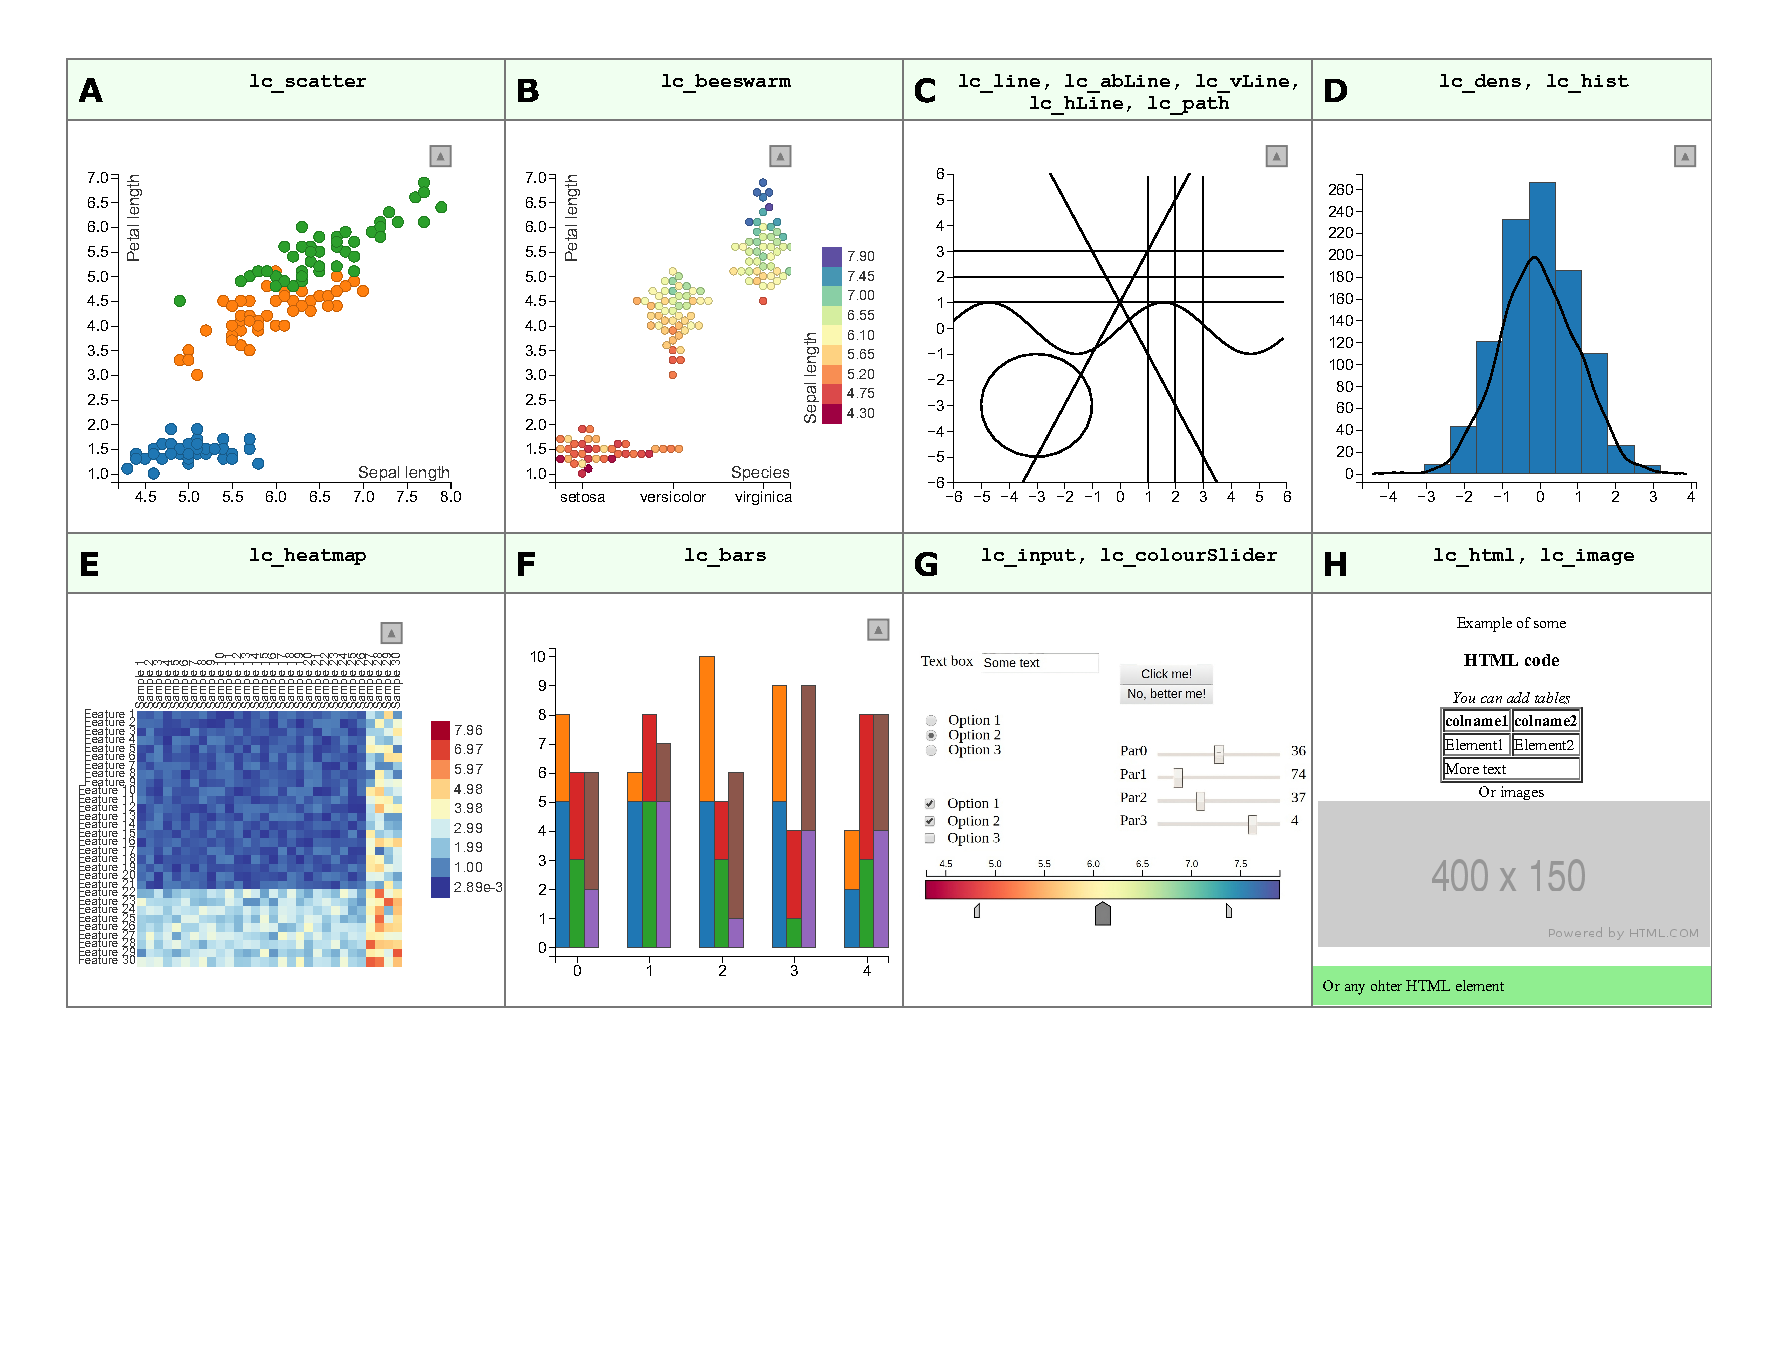
\includegraphics[width=\textwidth]{FigA/figA.png}
	\caption{Gallery of all available plotting functions the in \mintinline{R}{rlc} package. A scatter plot (a); a bee swarm plot (based on d3-beeswarm plugin [reference]) (b); a collection of various line plotting functions (c); a histogram and a density plot (density was multiplied by a factor of 500 to be visible on the same plot as the histogram) (d); a heatmap (e); a bar chart (f); a collection of elements to gather input from user (g); a function to add custom HTML code to the page (h). All this examples with code to create them can be found in the supplement.}
	\label{FigA}
\end{figure*}

R/LinkedCharts syntax is very similar to most commonly used plotting libraries. There is a set of 14 main functions - each responsible for a specific type of chart (such as scatter plot, heatmap, bar plot, etc.) or a navigation element (such as sliders or text fields). Figure \ref{FigA} shows them all together with some basic examples. Each plot is defined by its properties: some of them are required (such as \mintinline{R}{x} and \mintinline{R}{y} for a scatter plot or \mintinline{R}{value} for a heatmap) many others are optional (\mintinline{R}{palette}, \mintinline{R}{title}, \mintinline{R}{ticks} etc.). A full list of all the properties with live examples is available at \url{https://anders-biostat.github.io/linked-charts/rlc/tutorials/props.html} and also on the R man page for each plotting function. Many of the properties accept minor variations in spelling (\mintinline{R}{colour/color} or \mintinline{R}{labels/label}).

\begin{figure*}
	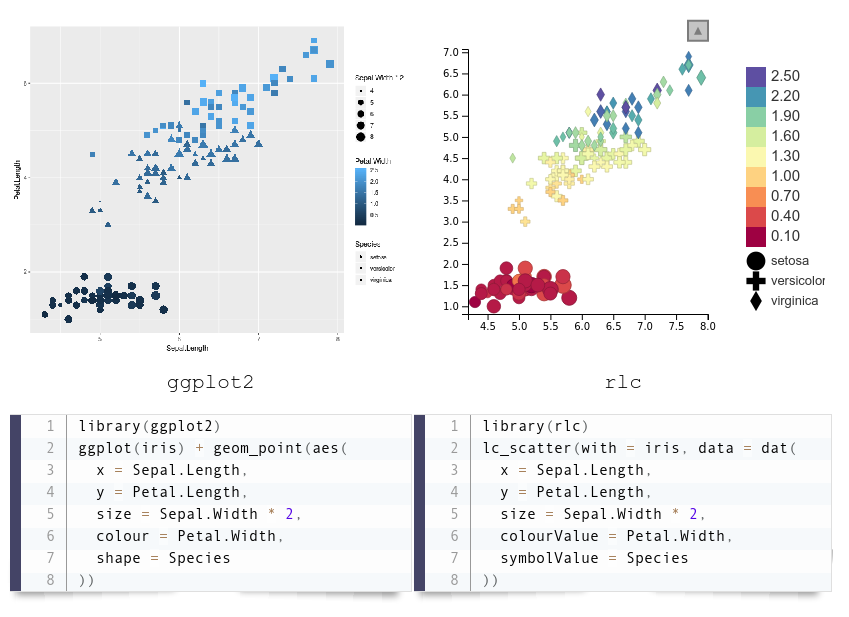
\includegraphics[width=\textwidth]{FigB/figB.png}
	\caption{Typical syntax of a R/LinkedCharts plot and its comparison with ggplot2 [ref] library as an example of one of the most commonly used plotting libraries. Lines of code are arranged so that same aspects of the charts are set next to each other. ``iris'' dataset, which is one the R built-in datasets, was used for this example. Both pieces of code are fully functional and their output is shown above the code.}
	\label{FigB}
\end{figure*}

The same structure with some minor differences in syntax is common for many generally used in research field plotting libraries. For instance, in Figure \ref{FigB} a comparison between \mintinline{R}{ggplot2} and \mintinline{R}{rlc} syntax is shown for making a simple scatter plot. As one can see, there is hardly any differences there. An important thing to notice here is the \mintinline{R}{dat} function, which plays the key role in R/LinkedCharts. Any property, defined inside this function, can be reevaluated at any moment simply by calling the \mintinline{R}{updateCharts} function. The corresponding plot will be then redrawn accordingly to the current state of the environment.

To make it more clear, let us imagine that we have a matrix \mintinline{R}{countMatrix} with some single-cell RNA-seq experiment results. Each row of the matrix is a gene, each column is a cell and values are numbers of reads from given gene detected in a given cell. Now we want to plot gene expression in two cells against each other and we have index of one of them stored in a variable named \mintinline{R}{cell1} and of the second one in \mintinline{R}{cell2}. To do this in R/LinkedCharts one should write the following code:

\begin{minted}{R}
lc_scatter(dat(x = countMatrix[, cell1], 
   y = countMatrix[, cell2]))
\end{minted}

If now values of \mintinline{R}{cell1} and \mintinline{R}{cell2} are changed, calling the \mintinline{R}{updateCharts} function will change the scatter plot to show gene expression in these new cells. The only thing that is missing now to make an interactive app is a reaction to mouse events on the web page. To this end, R/LinkedCharts provides a set of callback functions for the most common mouse events. They are all arguments with names spelled as \mintinline{R}{on_`eventName`} and a list of available listeners can differ between different chart types. A full list can be found on R man pages for each plotting function.

The most often used callback function is \mintinline{R}{on_click}. It is called every time an element of a chart (point, line, bar, cell) is clicked. A an argument this function gets index of the clicked element or two indices - for a row and a column in case of a heatmap. Let's extend our example to demonstrate the use of the \mintinline{R}{on_click} callback. Based on the above mentioned \mintinline{R}{countMatrix}, we can calculate some distance or correlation matrix to explore cell-to-cell similarities. For demonstration purposes, distances can be obtained in a very straightforward manner.

\begin{minted}{R}
distMatrix = as.matrix(dist(countMatrix))
\end{minted}

Now, next to the scatter plot of gene expressions in the two selected cells, we can have a heatmap of distances which is also used for navigation through all the pairs of cells. 

Code for such a minimalistic, but already fully functional interactive app is presented below:

\begin{minted}{R}
lc_heatmap(value = distMatrix, 
   on_click = function(d) {
      cell1 <<- d[1]
      cell2 <<- d[2]
      updateCharts()
})
lc_scatter(dat(x = countMatrix[, cell1],
	y = countMatrix[, cell2]))
\end{minted}

You can find the app produced by this code in the supplement alongside with a more nicely looking version.

In this example we use the \mintinline{R}{on_click} callback function to change the state variables \mintinline{R}{cell1} and \mintinline{R}{cell2} and to redraw the scatter plot. As it was previously mentioned, properties \mintinline{R}{x} and \mintinline{R}{y} will be reevaluated using the current values of the state variables, thus making it easy to keep charts up-to-date and ensure interactive behavior.

This basic example illustrates the main idea behind the LinkedCharts library. We define a set of charts employing a collection of variables to specify current state of the chart, i.e. selected cells, genes, samples, color labels, etc. With the help of the mouse event callback functions we change the state variables and call the \mintinline{R}{updateCharts} function to put the charts in accordance with their new values. This process is what "linked" in "LinkedCharts" stands for. We link several charts together by the means of \mintinline{R}{on_click} and other callback functions and updating charts. Though quite simple, this structure can produce powerful interactive apps for various research purposes.

The app from the example can be further customized by changing colours, shapes and sizes or adding meaningful labels and titles. Some technical aspects can be changed as well for better performance. For instance, we can specify what exactly should be redrawn on each \mintinline{R}{updateCharts} call and prevent meaningless updates of the heatmap. Please, check the supplement for a prettified version of the app with all necessary explanations.

\subsection{Use Cases}
\subsubsection{Quality check}

It is common that on the way from obtaining raw data towards meaningful conclusions one undertakes a number of steps each involving some data condensing and inevitable information loss. For example, raw reads in RNA-seq are aligned and counted to produce gene expression levels for each sample. However, quality of reads and confidence of alignment is no longer included in the data. If now researcher is interested in clusters of samples and other patterns such as trajectories, the next step may be to calculate a distance matrix. This will make data even more interprateable, but now we loose gene expression values. 

Of course, information that is put aside is not only used to produce the next step values, but also to perform various quality checks. Low-quality reads are usually removed from the study as well as samples that show abnormal expression patterns. We tend to believe that we no longer care about those pieces of data that are left behind in the research flow, since we've already taken everything we need from them. Yet, especially in studies involving big data, these checks are automated. The researcher only looks at some summarized reports and may also have a look at some random examples. If those look reasonable, the general assumption is that all the data that was not filtered out is also reasonable. However, while there is only one thing of everything being right, there are numerous ways for the data to be either wrong or just to be not like one has expected. Therefore, it's important to be able to look back, before making any kind of conclusions from a figure that show a condenced result.

This idea is the main motivation behind the LinkedCharts library. It is illustrated in the Figure \ref{FigC}. If we have a workflow or a pipeline, that performs certain transformations of the data, LinkedCharts offers an easy way to look back through each of the steps. Whenever a researcher encounters an interesting or suspicious pattern in the data, he or she can with minimal effort check that whether it real biological finding or some technical artifact, missed by quality checks. 

\begin{figure*}
	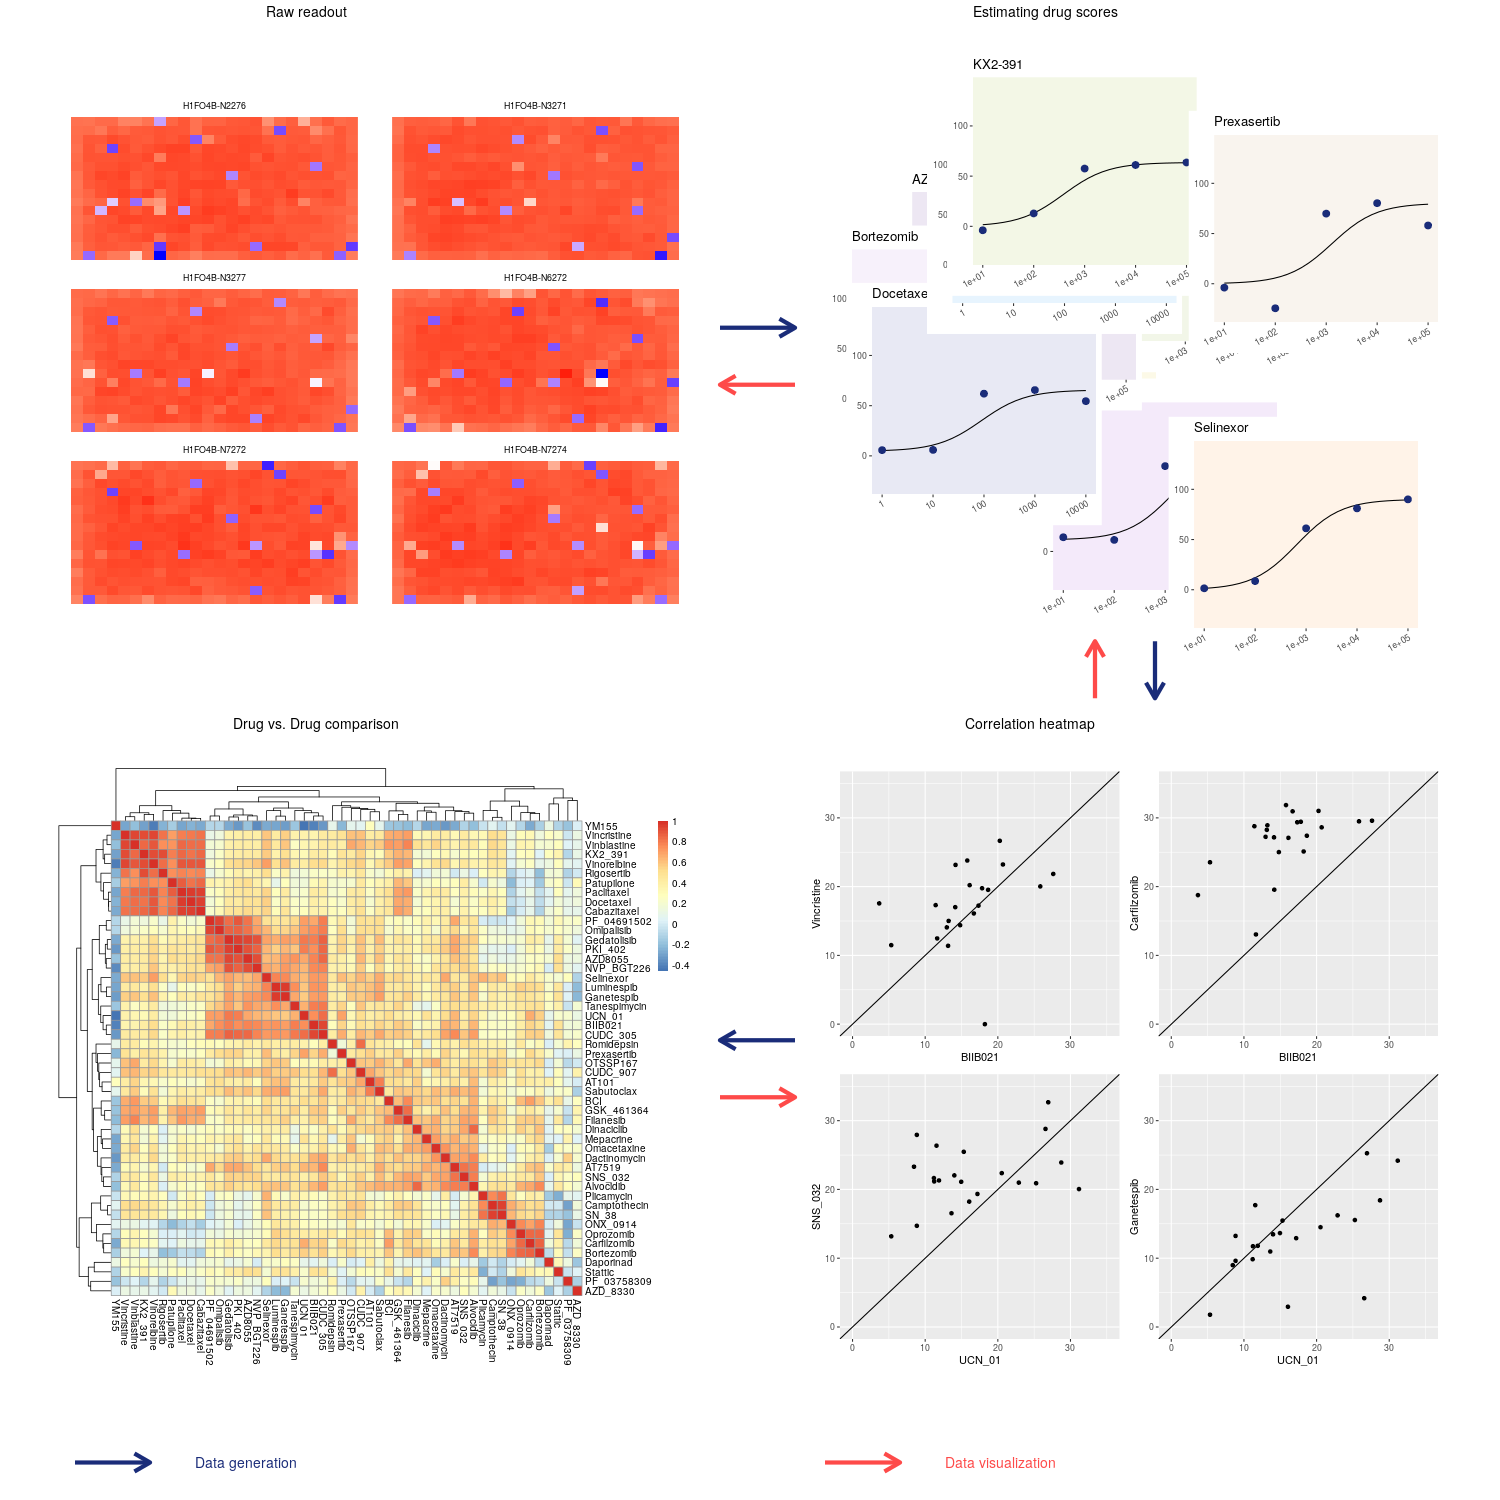
\includegraphics[width=\textwidth]{FigC/figC.png}
	\caption{Main idea behind the LinkedCharts library is shown based on a drug screening experiment. Blue arrow shows a direction of a common pipeline. We start with reading intensity values from plates with different cell lines, grown in the presence of a number drugs in different concentrations (A). These values are then normalized and aggregated to yield a single score for each drug (B). The scores of different drugs are compared to each other across all the tested cell lines (C). A drug-drug correlation heatmap is then produced to identify clusters of similar drugs (D). This pipeline is a simplified version of study from [reference? Have they published that by now?] for demonstration purposes. The live app and related code can be found in the supplement.}
	\label{FigC}
\end{figure*}

R/LinkedCharts is particularly effective in generating a chain of connected (``linked'') charts, where a chart explains each element of the previous one. For example, in the app from the previous section, scatter plot explains each cell of the heatmap. When a cell is clicked, we can see all the expression values for the two selected samples and thus it "explains" the obtained distance value. We can continue the chain of charts and, for instance, add a chart that for a selected gene will show quality of all the reads for the two selected samples that were mapped to this gene.

Such an app would allow a quick and easy spot check of uncovered data patterns and can give researcher a better way to understand inner connections between the data. For instance, to what extent noise cab influence the signal or what scale of changes in the value of interest is typical to the data.

Another example is shown in Figure \ref{FigC} and also is available in the supplement. It is based on the data from [reference].
For demonstration purposes, we use only a subset of available data here to simulate a typical drug-screening pipeline. In this subset 50 drugs each in five different concentrations were tested against 17 (?? check that) pancreatic cancer cell lines. The main heatmap shows drug-drug correlation values. By clicking on a cell of the heatmap user selects two drugs and can check individual drug scores (?) of each of them against all the tested cell lines. The inhibition values were calculated based on drug activity in five tested concentrations. So the third plot shows all those activity levels for each conentration. Finally, one can also find raw readouts from the plates in order to check for plate-related effects if any. More details as well as code and links to download the data one can find in the supplement.

\subsubsection{Exploratory analysis}

While interactivity is already heavily used for presenting study results to the research community, with R/LinkedCharts we would like to emphasize its advantages for everyday exploratory analysis. Since the syntax of R/LinkedCharts is made to resemble popular R packages such as ggplot2, it is not much more effort to make an interactive app instead of a usual static plot or a collection of plots. This app may not look pretty as most plots one makes while exploring new data aren't. Yet such a quick and dirty solution allows the researcher to pick into the data in an interactive manner without spending time on deploying a propper app. Therefore, interactive apps can be made as often and easily as static plots.

To illustrate this, every live example in the supplement is shown in two versions. One contains bare minimum of code to produce working and useful app. This kind of apps can be easily written on-the-fly to facilitate current research steps. The other shows how to make those work-in-progress-apps more presentable. This, usually, takes more effort, but not much more than to prepare a usual static plot for a paper or a presentation.


The example is very similar to the one from the previous section. The state of the app is now stored in the \mintinline{R}{gene} variable. Whenever a point in the MA-plot is clicked, this varible is changed and the second plot is updated. Different colours are used to indicated gene with significantly different expression between tumour and normal tissue in the MA-plot and to show different tissue types in the expression plot. We've added the \mintinline{R}{openPage} function to add a table layout to the web page. This step is optional and allows us to put the two charts next to each other.

\subsubsection{Server apps}

So far, we've only talked about local apps, i.e. ones that are created by running script locally and are intended to be used by the person who made it. However, the same apps can also be run on the server and shared between multiple users. There is only one additional thing that is required to turn a local app into a server app: One needs to specify a list of local variables and their default values. Local variables are those that can be rewritten by several users independently. In most cases they are also state variables: i.e. variables that store current state of an app (selected genes, samples, etc.). Thus, to run the app from the previous section on a server, one would need just to replace the first two lines with

\begin{minted}{R}
openPage(layout = "table1x2", 
         sessionVars = list(gene = 1))
\end{minted}

Now a link to the app  can be shared and it can be accessed by multiple users simultaneously.

Of course, there are other things that can make a server app more customized. One can add some default content to each opened page, control each client session (and, for example, close those, that don't show any activity for considerable amount of time), limit memory usage or number of active connections simultaneously. Yet, all these parameters are optional. More information about possible options can be found on R man pages for classes \mintinline{R}{App} and \mintinline{R}{Session}.

\subsubsection{Stand-alone apps}

LinkedCharts can also be used to create stand-alone apps. This kind of apps do not rely on a running R session and thus can be directly sent to a collaborator or used as a supplement to a paper. To make such an app, one should use the JavaScript version of the LinkedCharts library and either load preprocessed data or perform all the calculations with JavaScript. 

For this kind of apps you don't need a server, but can directly send them to a collaborator as an HTML file that can be opened in any browser. The page will already contain all the data and interactive functionality. Yet to make such an app one should use a JavaScript version of the Linked-Charts library. We tried to make required level of experience with JavaScript to minimum and make necessary code understandable. For each example in the supplement we also provide the JavaScript code necessary to create the same app without running R session. More documentation on linked-charts.js as well as various tutorials are available at...

\subsection{Further customization}

\begin{small} 
\balance
\bibliography{lc}
\end{small}

\end{document}


